\documentclass[12pt]{article}

\usepackage[T1]{fontenc}
\usepackage[polish]{babel}
\usepackage[utf8]{inputenc}
\usepackage{lmodern} %zazwyczaj używam tej czcionki
%\usepackage{mathptmx} %times new roman
%\usepackage{helvet}
%\usepackage{amsmath}	%pakiet z symbolami matematycznymi
\usepackage{graphicx}	%do wstawiania rysunków
\usepackage{float}	%do umiejscowienia rysunków w dobrych miejscach
\usepackage{wrapfig} %do wstawiania obrazków obok tekstu
\usepackage{caption}
\usepackage{subcaption}
\usepackage{listings}  % do wstawiania kodu
%\usepackage{indentfirst}	%do zaczynania pierwszego akapitu wcięciem
%\usepackage{multirow}	%do tabel
\usepackage{hyperref}	%refy działają jak hyperlinki
\usepackage{caption}	%przy refie idze na góre obrazka
\usepackage{xcolor}
\selectlanguage{polish}	%język
\graphicspath{ {./obrazki/} }	%folder gdzie znajdują się rysunki
\hypersetup{
	colorlinks   = true, %Colours links instead of ugly boxes
	urlcolor     = blue, %Colour for external hyperlinks
	linkcolor    = blue, %Colour of internal links
	citecolor    = red %Colour of citations
}
\bibliographystyle{abbrv}
\renewcommand{\familydefault}{lmss}

\colorlet{punct}{red!60!black}
\definecolor{background}{HTML}{EEEEEE}
\definecolor{delim}{RGB}{20,105,176}
\colorlet{numb}{magenta!60!black}

\lstdefinelanguage{json}{
	basicstyle=\normalfont\ttfamily,
	numbers=left,
	numberstyle=\scriptsize,
	stepnumber=1,
	numbersep=4pt,
	showstringspaces=false,
	breaklines=true,
	frame=lines,
	backgroundcolor=\color{background},
	literate=
	*{0}{{{\color{numb}0}}}{1}
	{1}{{{\color{numb}1}}}{1}
	{2}{{{\color{numb}2}}}{1}
	{3}{{{\color{numb}3}}}{1}
	{4}{{{\color{numb}4}}}{1}
	{5}{{{\color{numb}5}}}{1}
	{6}{{{\color{numb}6}}}{1}
	{7}{{{\color{numb}7}}}{1}
	{8}{{{\color{numb}8}}}{1}
	{9}{{{\color{numb}9}}}{1}
	{:}{{{\color{punct}{:}}}}{1}
	{,}{{{\color{punct}{,}}}}{1}
	{\{}{{{\color{delim}{\{}}}}{1}
	{\}}{{{\color{delim}{\}}}}}{1}
	{[}{{{\color{delim}{[}}}}{1}
	{]}{{{\color{delim}{]}}}}{1},
}

\title{Komunikacja człowiek komputer - sprawozdanie z aplikacji Mask Detector}
\author{Gorgoń Adam - 145278\\Grochowska Paulina - 145284}
\begin{document}
	\maketitle
	
	\section{Wstęp}
	Celem projektu jest zaimplementowanie aplikacji do wykrywania, czy osoba ma założoną maskę ochronną. Podczas tworzenia projektu wgłębiliśmy się nie tylko w metody wykrywania twarzy, maski, lecz także w miarę potrzeby poszerzyliśmy swoją wiedzę o strukturze i sposobie działania sieci neuronowej.
	\section{Prezentacja aplikacji}
	\begin{figure}
		\centering
		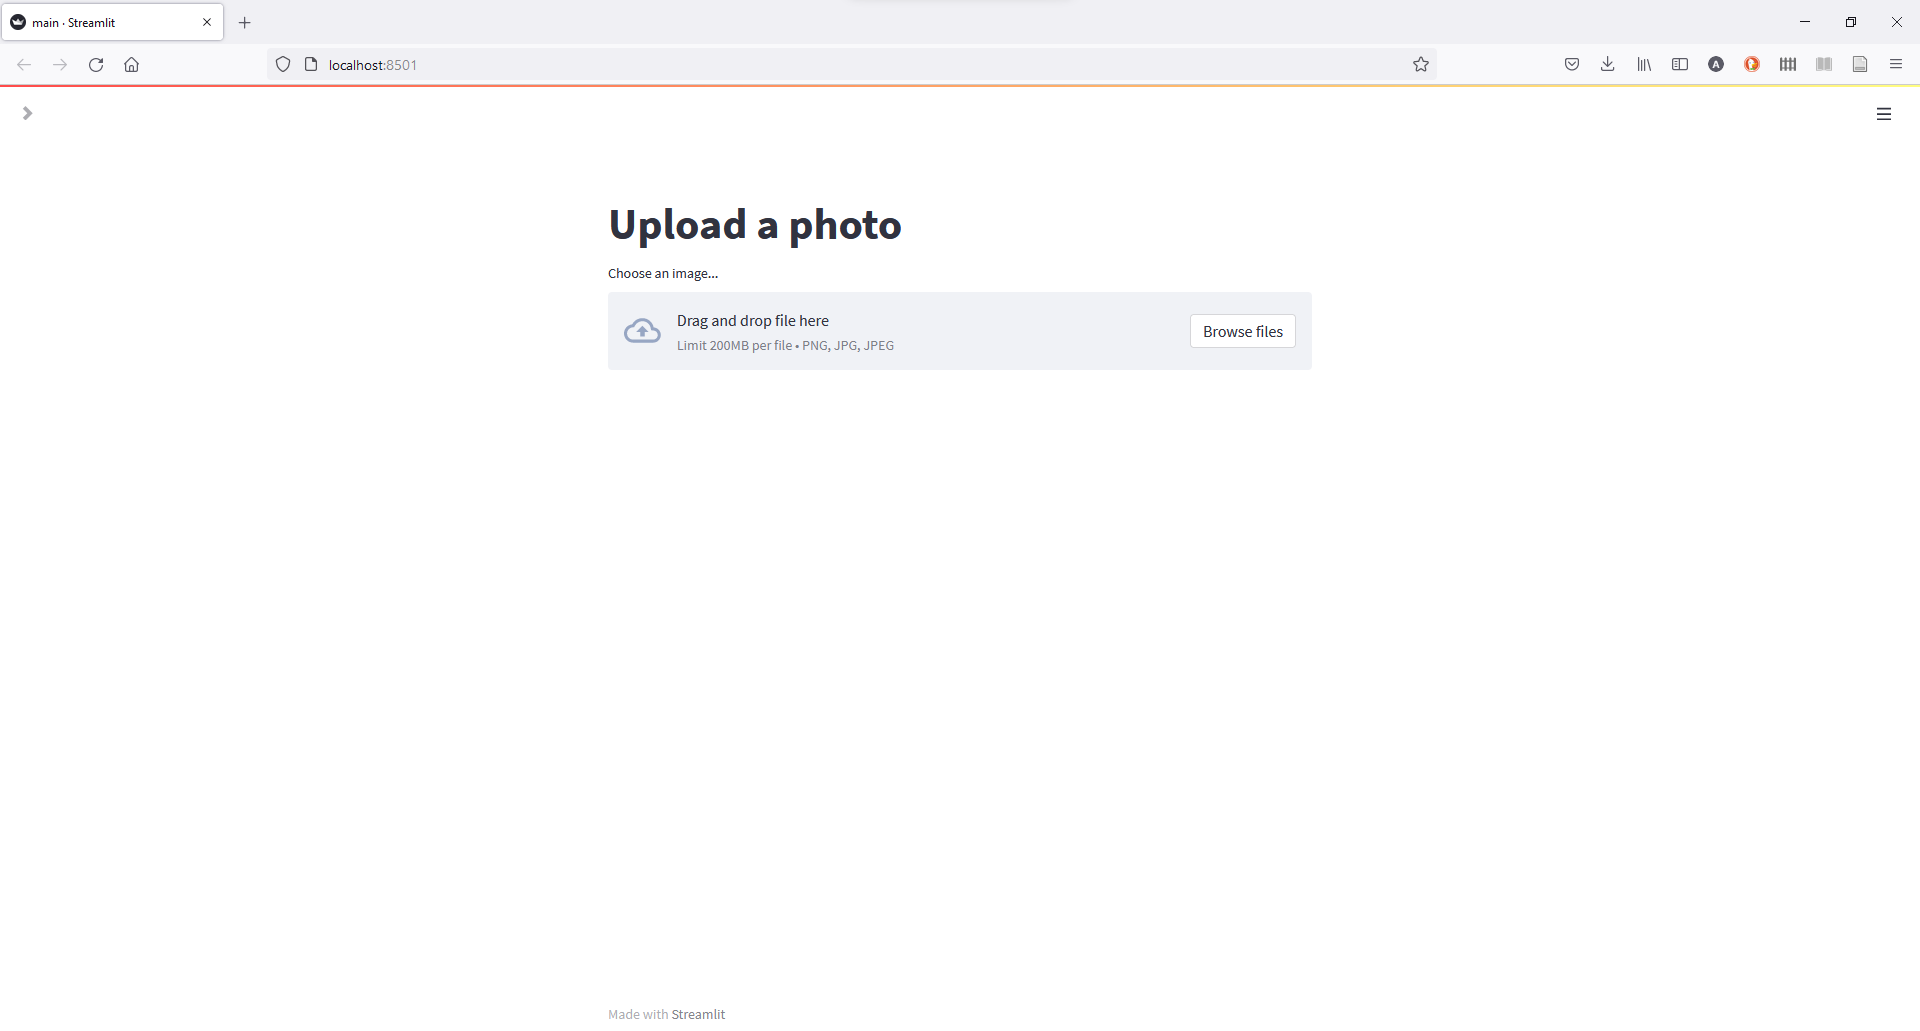
\includegraphics[width=\textwidth]{apka.png}
		\caption{Aplikacja po otworzeniu}
		\label{fig:apka}
	\end{figure}
	Po włączeniu aplikacji webowej na ekranie pojawia się przycisk, który umożliwia wgranie wcześniej przygotowanego zdjęcia. Po użyciu komponentu pojawia się okno menedżera plików. Po wybraniu i zatwierdzeniu zdjęcia o formacie .jpg, .jpeg lub .png okno zamyka się, a aplikacja zaczyna przetwarzanie obrazu. Po paru sekundach w przeglądarce pojawia się nasze zdjęcie z modyfikacjami.
	
	Pierwszą z nich jest kolorowa ramka wskazująca na lokalizację twarzy. Może ona wystąpić w dwóch wariantach kolorystycznych: czerwonej lub zielonej. Czerwona oznacza, że po przetworzeniu zdjęcia przez sieć neuronową uznano, iż osoba na zdjęciu nie posiada założonej maseczki ochronnej. W przeciwnym razie, ramka staje się zielona. Dodatkowo nad tym prostokątem można znaleźć informację słowną o posiadaniu (‘Mask’) lub braku maseczki (‘No Mask’) w kolorze odpowiadającym kolorze ramki.
	
	Następną rzeczą są dwie wartości liczbowe oddzielone znakiem ‘/’ zlokalizowane na lewo od napisu. Liczba znajdująca się na lewo od znaku oznacza pewność wykrycia twarzy przez model wykorzystany w algorytmie. Mieści się ona w zakresie \([0, 1]\). Natomiast druga liczba oznacza wartość zwróconą przez sieć neuronową. Dotyczy ona pewności wykrycia maseczki i także mieści się w zakresie \([0, 1]\).
	\section{Dane}
	Zbiór danych użytych do trenowania i walidacji modelu pochodzi ze strony \href{https://www.kaggle.com/wobotintelligence/face-mask-detection-dataset}{Kaggle}. Składa się na niego dokładnie 5749 zdjęć, a na każdym z nich znajduje się co najmniej jedna osoba.
	
	W pliku submission.csv znajduje się tabela z nazwą zdjęcia, koordynatami jednej lub wielu twarzy osoby oraz co najmniej jedną etykietą opisującą osobę/y. Wśród nich:
	\begin{itemize}
		\item 'face\_with\_mask',
		\item 'mask\_colorful',
		\item 'face\_no\_mask',
		\item 'face\_with\_mask\_incorrect',
		\item 'mask\_surgical',
		\item 'face\_other\_covering',
		\item 'scarf\_bandana',
		\item 'eyeglasses'.
	\end{itemize}
	Jednak korzystaliśmy jedynie z dwóch z nich: ‘face\_with\_mask', 'face\_no\_mask'. W konsekwencji otrzymaliśmy 4180 zdjęć osób w maskach oraz 1569 zdjęć osób bez masek.
	
	Sprawą niezbalansowanych danych zajęliśmy się przy trenowaniu modelu.
	Dodatkowo do każdego elementu zbioru znajdował się plik .json. Pomógł on w sprawniejszym i dokładniejszym przetworzeniu każdego pliku.
	\begin{figure}[h]
		\centering
		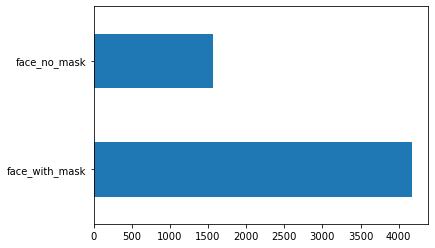
\includegraphics[width=\textwidth]{dane.png}
		\caption{Wykres przedstawiający ilość danych}
		\label{fig:dane}
	\end{figure}
	\begin{lstlisting}[language=json,caption=Przykład pliku json, captionpos=b]
{'FileName': '1801.jpg',
	'NumOfAnno': 1,
	'Annotations': [{'isProtected': False,
		'ID': 924868908868875136,
		'BoundingBox': [451, 186, 895, 697],
		'classname': 'face_no_mask',
		'Confidence': 1,
		'Attributes': {}}]}
	\end{lstlisting}
	\section{Użyte modele}
	Do wykrywania twarzy użyliśmy wytrenowanego modelu z biblioteki \href{https://opencv.org/}{OpenCV} w frameworku Caffe\cite{jia_caffe_2014}. Do klasyfikacji, czy osoba posiada maskę stworzyliśmy własną się konwolucyjną zbudowaną na technologi tensorflow\cite{tensorflow2015-whitepaper}. Model trenował się na cpu 3 godziny. Wczytywał zdjęcia z wcześniej wspomnianej bazy. Proporcje zbioru treningowego do testowego, wynosiły 0.8/0.2. Do lepszego wytrenowania model generował sobie zdjęcia, obracając zdjęcia o maksymalnie 15 stopni, robiąc lustrzane odbicie oraz przesuwając w pionie lub poziomie o 0.1 zdjęcia.
	\section{Działanie programu}
		\subsection{Przygotowanie zdjęcia do modelu}
		Wczytane zdjęcie jest zmieniane na tablicę jako RBG. Następnie układ jest zmieniany na BGR. Wynika to z faktu, że podczas trenowania dane były wczytywane za pomocą biblioteki \href{https://opencv.org/}{OpenCV}(wczytuje bgr), a w aplikacji przez \href{https://pillow.readthedocs.io/en/stable/}{Pillow}(wczytuje rgb).
		
		Następnie rozjaśniamy obraz za pomocą korekcji gamma, by zmniejszyć efekt cienia na zdjęciu.
		\begin{figure}
			\centering
			\begin{subfigure}[b]{0.49\textwidth}
				\centering
				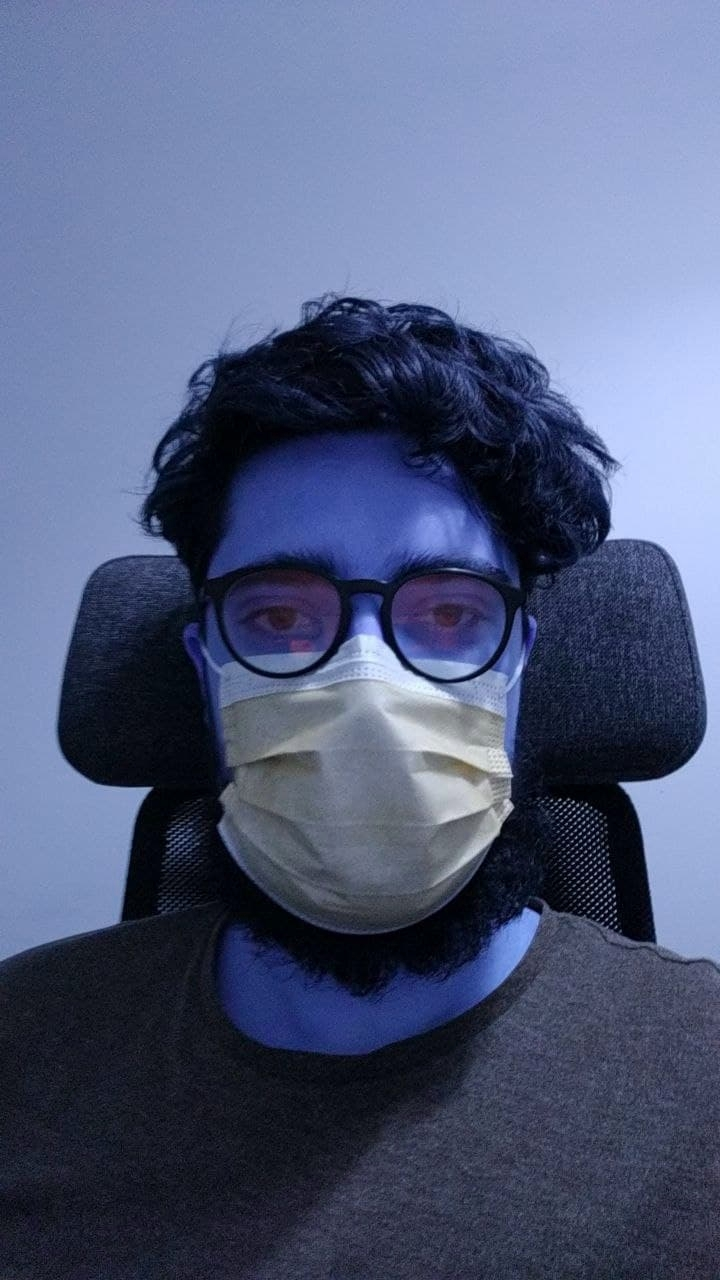
\includegraphics[width=0.45\textwidth]{rgb_to_bgr.jpeg}
				\caption{Zdjęcie bez obróbki z źle wczytanymi kolorami}
				\label{fig:bgr}
			\end{subfigure}
			\hfil
			\begin{subfigure}[b]{0.49\textwidth}
				\centering
				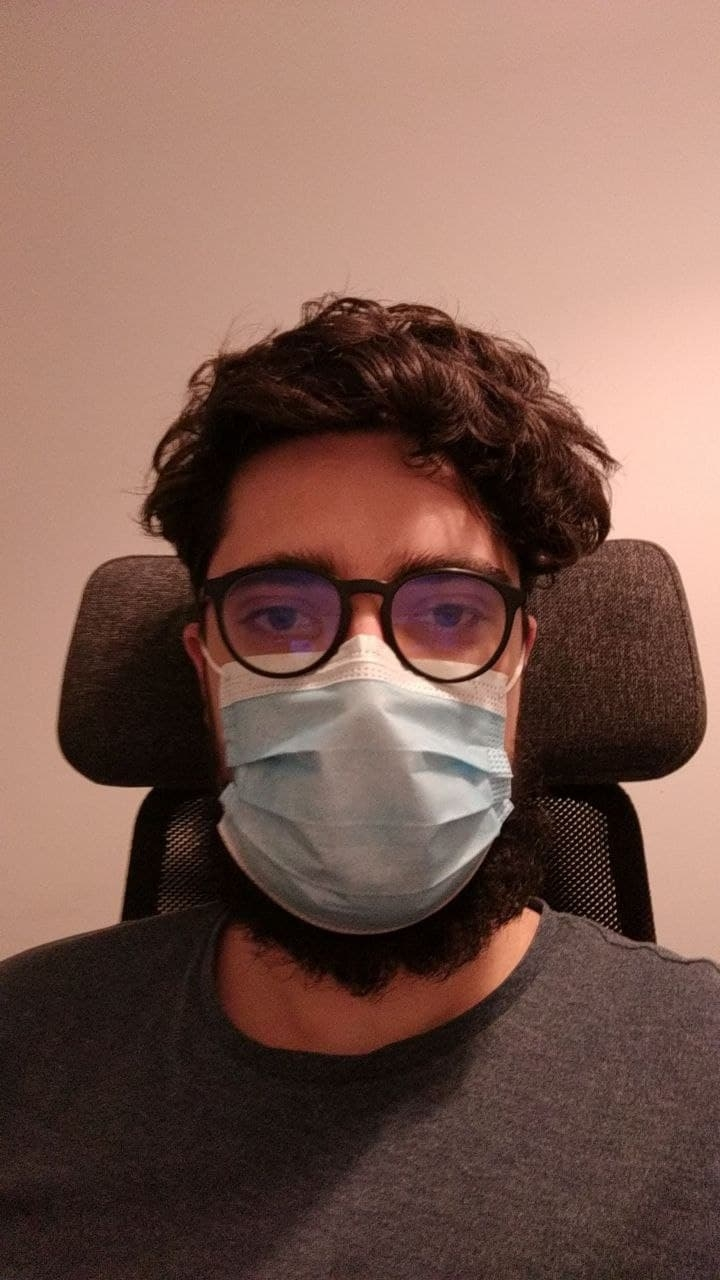
\includegraphics[width=0.45\textwidth]{nieprzerobione.jpeg}
				\caption{Zdjęcie bez obróbki z dobrze wczytanymi kolorami}
				\label{fig:nieprzerobione}
			\end{subfigure}
			\caption{Wczytywanie zdjęcia}
		\end{figure}
		\begin{figure}
			\centering
			\begin{subfigure}[b]{0.49\textwidth}
				\centering
				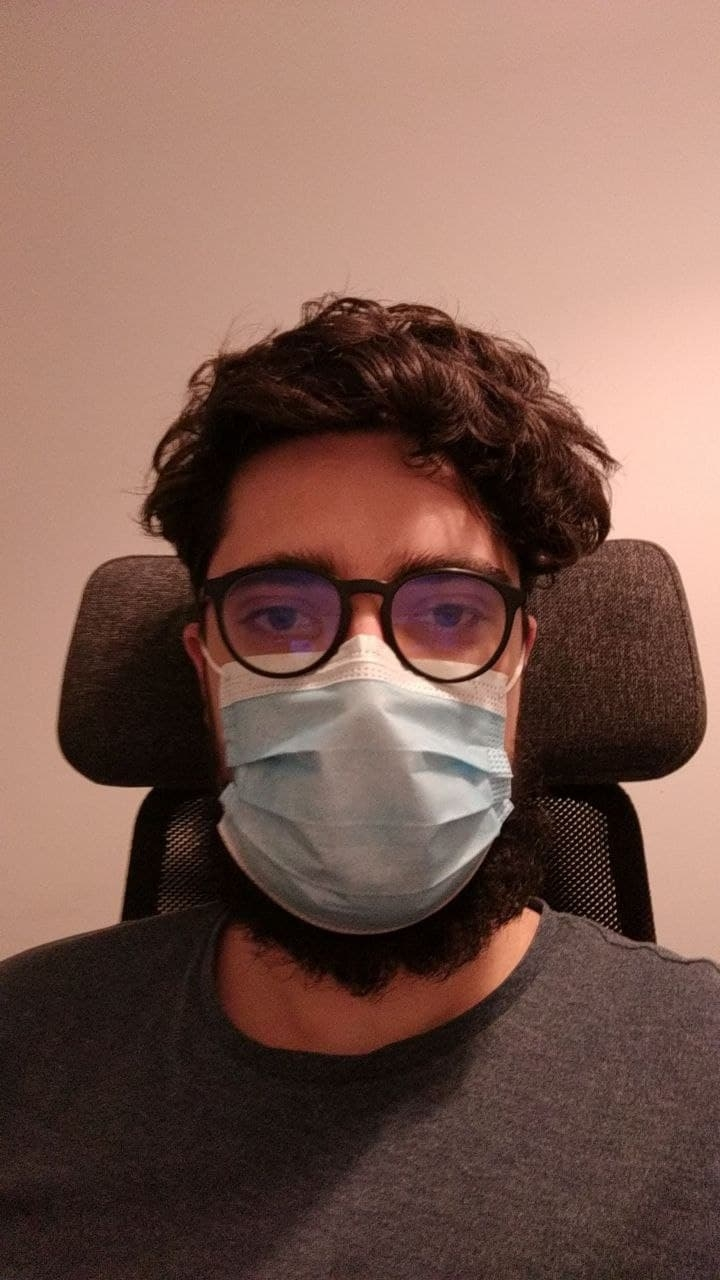
\includegraphics[width=0.45\textwidth]{nieprzerobione.jpeg}
				\caption{Przed}
				\label{fig:przed_gamma}
			\end{subfigure}
			\hfil
			\begin{subfigure}[b]{0.49\textwidth}
				\centering
				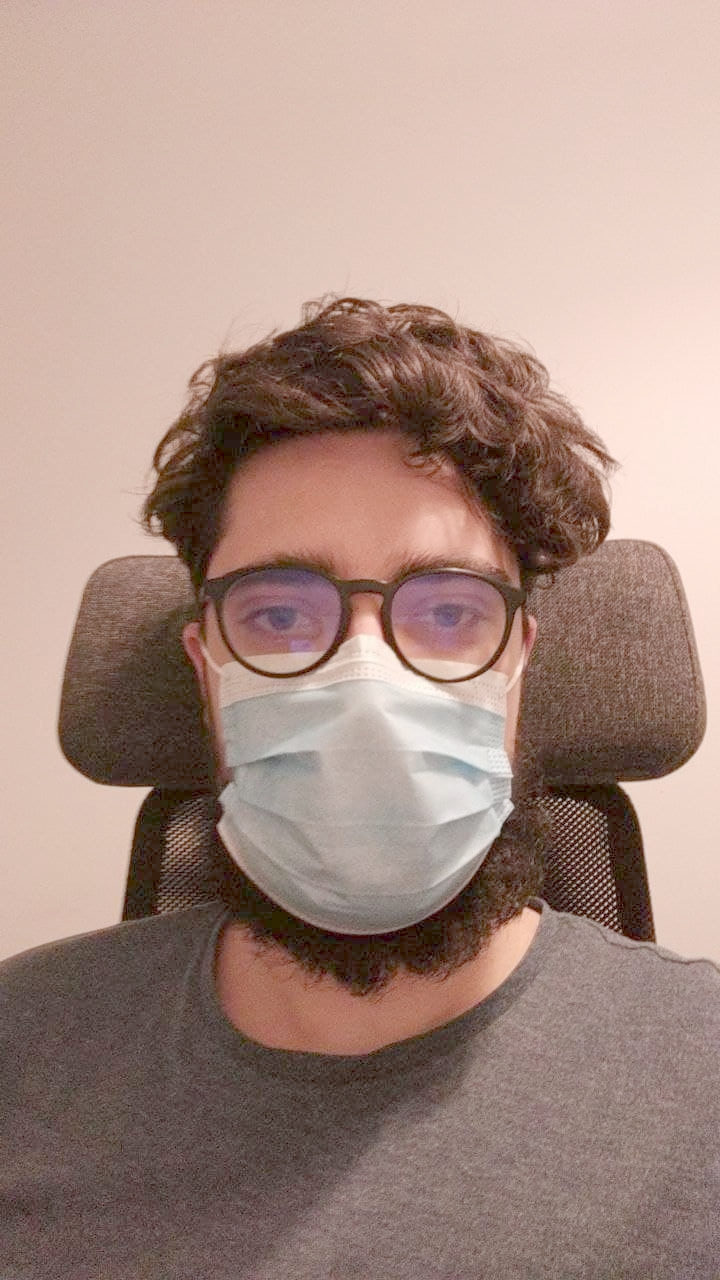
\includegraphics[width=0.45\textwidth]{po_gamma.jpeg}
				\caption{Po}
				\label{fig:po_gamma}
			\end{subfigure}
			\caption{Korekcja gamma}
		\end{figure}
		\subsection{Detekcja twarzy}
		Model sprawdza na zdjęciu czy znajduję się twarz. Jeśli pewność algorytmu na to, że w przeszukiwanym w tym momencie prostokącie znajduje się twarz, wynosi ponad 0.5, to program przechodzi do klasyfikacji.
		\subsection{Klasyfikacja twarzy}
		Jeśli program znajdzie twarz, to "wycina" prostokąt uznany za twarz, zmienia jego rozmiar na 124x124 i wysyła do sieci konwolucyjnej. Sieć wyrzuca liczbę w zakresie \([0, 1]\). Jeśli liczba jest mniejsza od 0.5, to twarz ma na sobie założoną maskę, w przeciwnym razie algorytm uznaje, że na twarzy nie ma maseczki.
		\begin{figure}[h]
			\centering
			\begin{subfigure}[b]{0.49\textwidth}
				\centering
				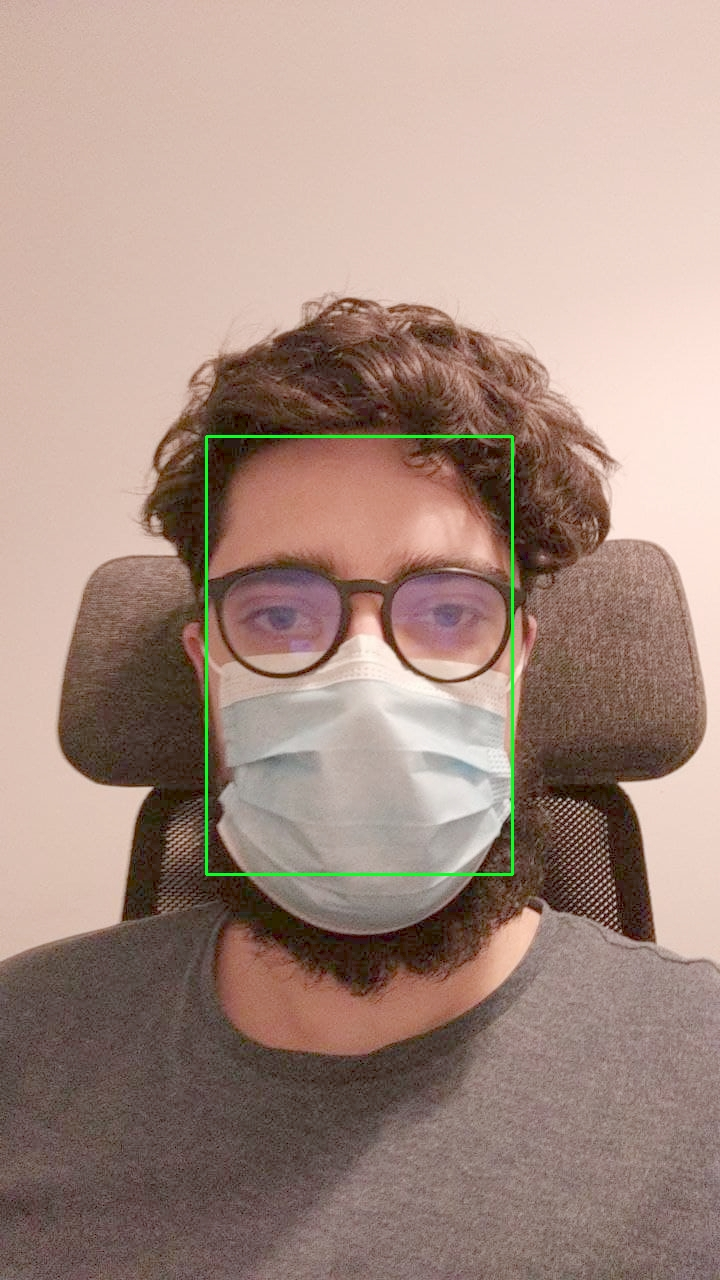
\includegraphics[width=0.45\textwidth]{twarz.jpeg}
				\caption{Algorytm znalazł twarz}
				\label{fig:twarz}
			\end{subfigure}
			\hfil
			\begin{subfigure}[b]{0.49\textwidth}
				\centering
				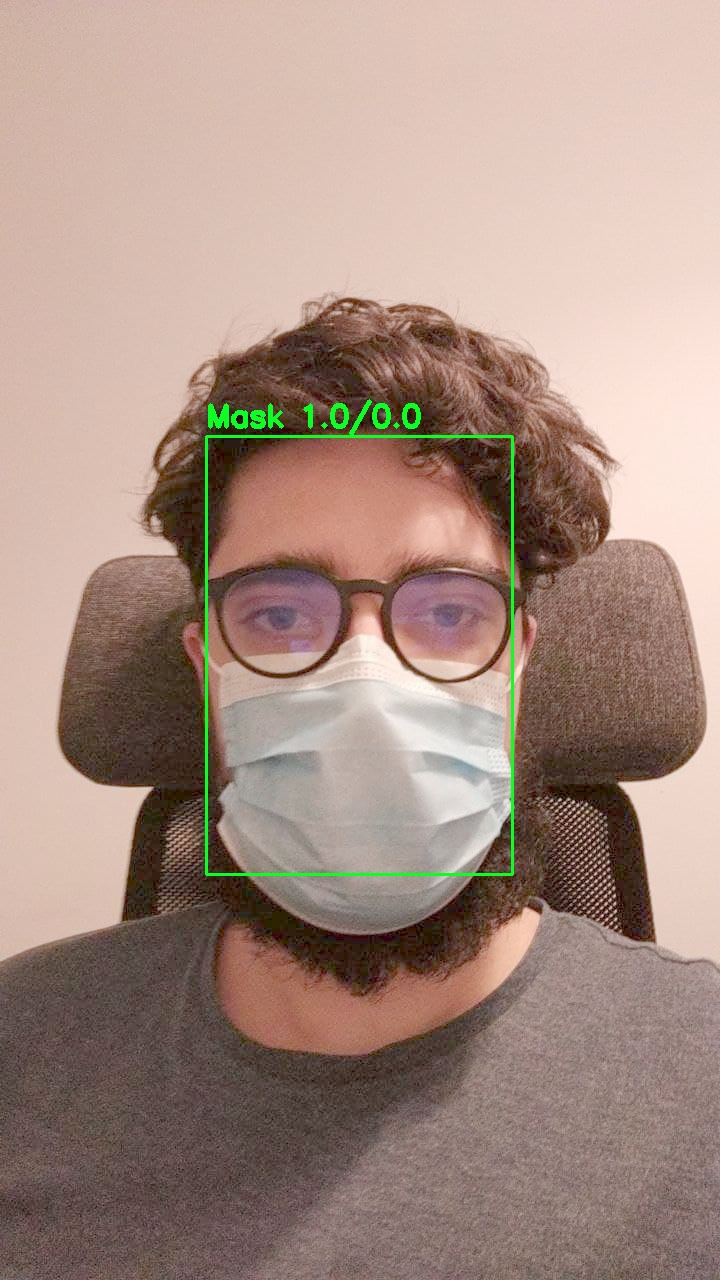
\includegraphics[width=0.45\textwidth]{maska.jpeg}
				\caption{Algorytm sklasyfikował twarz}
				\label{fig:maska}
			\end{subfigure}
			\caption{Działanie modelu}
		\end{figure}
	\section{Podsumowanie}
	Po wytrenowaniu modelu i sprawdzeniu działania aplikacji przeanalizowaliśmy otrzymane wyniki i doszliśmy do następujących wniosków.
	Zdecydowana większość uzyskanych wartości była zgodna z oczekiwanymi (macierz pomyłek, wykres \ref{fig:conf}). Wystąpienie niepoprawnych dopasowań może wynikać z nieidealnego dobrania parametrów. Niemniej jednak przy zastosowaniu sieci neuronowych obecność błędów jest normalna, a uzyskana pewność jest zadowalająca na skalę, ograniczenia pamięciowe i czasowe aplikacji.
	
	Ponadto patrząc na wykres \ref{fig:accidents} widać, że dla wartości parametru granicznego równego 0.5 otrzymujemy minimum funkcji. Oznacza to, że parametr o tej wartości zapewnia nam najmniejszą ilość pomyłek, a przy tym najlepsze rezultaty.
	
	Analizując wykresy \ref{fig:accuracy} i \ref{fig:loss} można dojść do wniosku, że krzywa odpowiadająca za dane testowe walidacyjne szybko ‘zbliżyła się’ do do drugiej krzywej. Wskazuje to na szybką poprawę efektywności sieci neuronowej, a także na ogólną dobrą jakość programu.
	\begin{figure}[H]
		\centering
		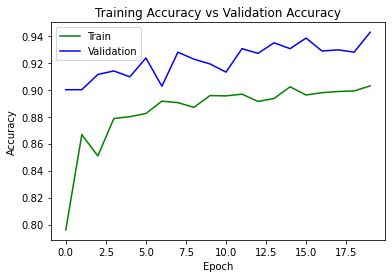
\includegraphics[width=0.8\textwidth]{accuracy.png}
		\caption{Wykres przedstawiający dokładność na danych walidacyjnych i treningowych}
		\label{fig:accuracy}
	\end{figure}
	\begin{figure}[H]
		\centering
		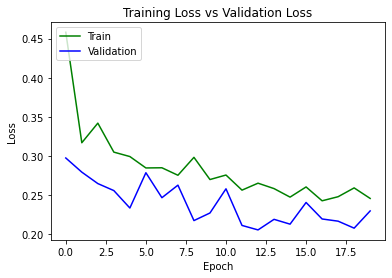
\includegraphics[width=0.8\textwidth]{loss.png}
		\caption{Wykres przedstawiający straty na danych walidacyjnych i treningowych}
		\label{fig:loss}
	\end{figure}
	\begin{figure}[H]
		\centering
		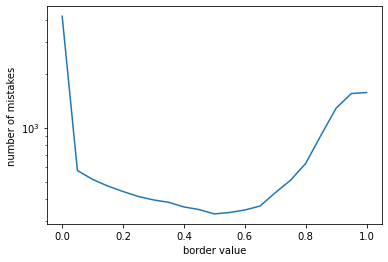
\includegraphics[width=0.8\textwidth]{accidents.png}
		\caption{Wykres przedstawiający ilość pomyłek, przy zmianie parametru granicznego}
		\label{fig:accidents}
	\end{figure}
	\begin{figure}[H]
		\centering
		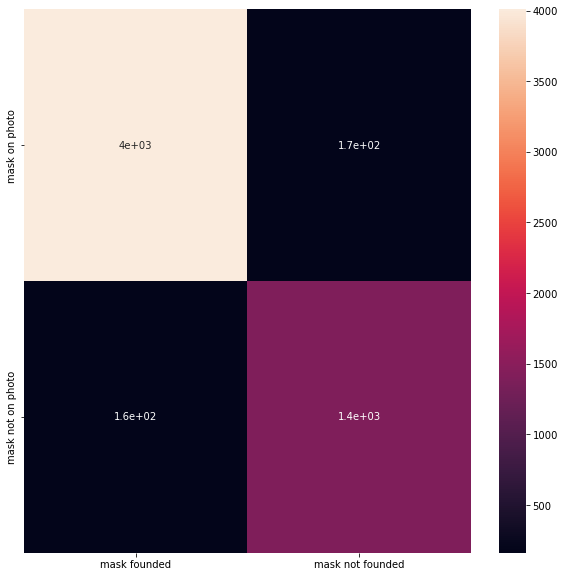
\includegraphics[width=0.6\textwidth]{conf.png}
		\caption{Macierz pomyłek dla parametru granicznego o wartości 0.5}
		\label{fig:conf}
	\end{figure}
	\newpage
	\bibliography{md_bibl.bib}
\end{document}